\documentclass{beamer}

\setbeamertemplate{footline}[frame number]

\usepackage{multimedia}

\usepackage{amsmath}
\usepackage{amsfonts}

\usepackage{apacite}

\usepackage{graphicx}
\graphicspath{{data/}}

\usepackage{pgfplots}
\usepackage{tikz}
\usetikzlibrary{arrows, shapes, fit, decorations.markings}

\tikzstyle{vecArrow} = [thick, decoration={markings,mark=at position
   1 with {\arrow[semithick]{open triangle 60}}},
   double distance=1.4pt, shorten >= 5.5pt,
   preaction = {decorate},
   postaction = {draw,line width=1.4pt, white,shorten >= 4.5pt}]
\tikzstyle{innerWhite} = [semithick, white,line width=1.4pt, shorten >= 4.5pt]

\makeatletter
  \def\inputTikZ{\@ifnextchar[{\@with}{\@without}}
  \def\@with[#1]#2{
    \begingroup
      \tikzset{every picture/.style={scale=#1}}
      \input{data/#2.tikz}
    \endgroup
  }
  \def\@without#1{\input{data/#1.tikz}}
\makeatother

\newcommand{\TODO}[1]{\emph{\small{{\bf TODO: } #1}}}

\newcommand{\etal}{\textit{et al. }}
\newcommand{\etc}{\textit{etc. }}
\newcommand{\eg}{\textit{e.g. }}

\title{Multi-Sensory Integration : Theories, Observations and Neural Implementation}
\author{Weipeng He \\ \texttt{2he@informatik.uni-hamburg.de}}
\date{July 5, 2013}

\begin{document}

\frame{\titlepage}

\begin{frame}
\frametitle{Outline}
\tableofcontents
\end{frame}

\section{Introduction}
\begin{frame}
  \frametitle{Introduction}
  \begin{itemize}
    \item ``Multisensory integration'' is the process of combining sensory cues of different modality.
    \item Multi-modal senses provide complementary information.

    ~
    \item Examples:
    \begin{itemize}
      \item Visual-auditory integration for spatial localization.
      \item Visual-haptic integration for perceiving the size and position;
      \item Visual-vestibular integration for perceiving self-motion;
    \end{itemize}
  \end{itemize}
\end{frame}

\begin{frame}
  \frametitle{Ventriloquist effect}
  \begin{center}
    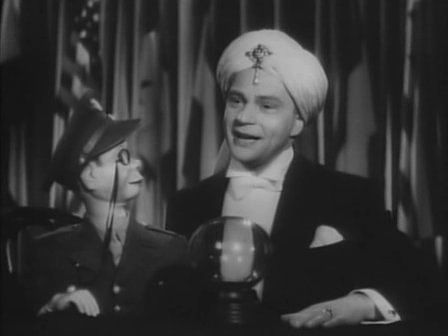
\includegraphics[width=.8\textwidth]{ventriloquism}
  \end{center}
\end{frame}

\begin{frame}
  \frametitle{Stream/bounce illusion}
  \begin{center}
    \movie[externalviewer=totem]{
\includegraphics[width=.6\textwidth]{streambounce}}{video/streambounce.mp4}
  \end{center}
\end{frame}

\begin{frame}
  \frametitle{Two major types of study}
  \begin{center}
    \inputTikZ[.9]{flow}
  \end{center}
  \begin{itemize}
    \item Psychophysics versus Neurophysiology.
    \item Behavioral versus Neuronal.
    \item How about the missing part?
  \end{itemize}
\end{frame}

\section{Psychophysics of Multisensory Integration}

\begin{frame}
  \frametitle{Psychophysics of multisensory integration}
  \begin{itemize}
    \item Study the relationship between multisensory stimuli and behavior response.

    ~
    \item Driven by statistical normative study, \eg optimal cue integration.
    \item A solution is called an ideal observer model.

    ~
    \item Psychophysical experiments are used for observation. 
    \item Human (as well as other animals) multisensory perception is indeed statistically optimal.
  \end{itemize}
\end{frame}

\begin{frame}
  \frametitle{Linear model for maximum reliability \cite{landy_ideal-observer_2011}}
  \begin{itemize}
    \item What is ``optimal''?
    \begin{itemize}
      \item Minimize uncertainty;
      \item \eg Maximize reliability (gain).
    \end{itemize}

    ~
    \item The best estimate is:
\begin{gather}
  \hat{S}_{opt} = \sum_{i=1}^{n} w_i \hat{S}_i \label{eq:optest} \\
  w_i = \frac{g_i}{\sum_{i=1}^{n} g_i}, \quad g_i = \frac{1}{\sigma_i^2} \label{eq:optweight}
\end{gather}
    \item where $\hat{S}_i, i=1 \dots n$ are the input cues, $\sigma_i$ are their variance.
    \item The gain of optimal estimate:
\begin{equation}
  g_{opt} = \sum_{i=1}^{n} g_i \label{eq:optrel}
\end{equation}
  \end{itemize}
\end{frame}

\begin{frame}
  \frametitle{Bayesian inference}
  \begin{itemize}
    \item The posterior probability
\begin{equation}
  p(s|c_1,c_2) = \frac{p(c_1,c_2|s)p(s)}{p(c_1,c_2)}
\end{equation}
    \item With a flat prior and independent cues
\begin{equation} \label{eq:post}
  p(s|c_1,c_2) \propto p(c_1|s)p(c_2|s)
\end{equation}
    \item With Gaussian noise, this product is also a Gaussian of which the mean and inverse of variance are consistent to Equation \ref{eq:optest} and \ref{eq:optrel} respectively. 
  \end{itemize}
  
  \begin{center}
    \inputTikZ[.7]{bayes}
  \end{center}
\end{frame}

\begin{frame}
  \frametitle{Behavioral experiments \cite{fetsch_bridging_2013}}
  \begin{center}
    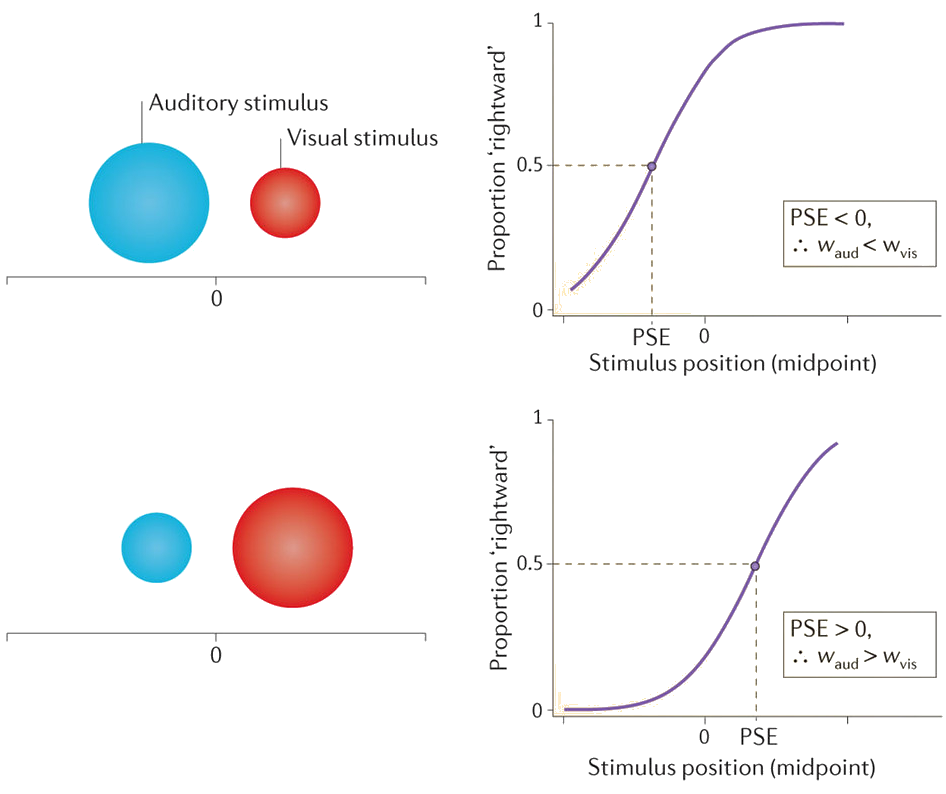
\includegraphics[width=.9\textwidth]{visaudloc1}
  \end{center}
\end{frame}

\begin{frame}
  \frametitle{Behavioral experiments \cite{fetsch_bridging_2013}}
  \begin{center}
    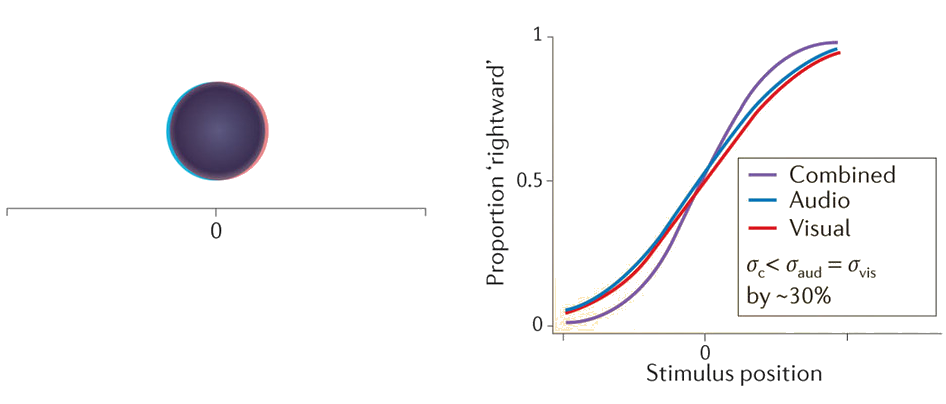
\includegraphics[width=.9\textwidth]{visaudloc2}
  \end{center}
  \begin{itemize}
    \item These results show that humans perform near-optimally in multisensory perception (with exceptions).
  \end{itemize}
\end{frame}

\section{Neurophysiology of Multisensory Integration}

\begin{frame}
  \frametitle{Neurophysiology of multisensory integration}
  \begin{itemize}
    \item Study the relationship between multisensory stimuli and neuronal response.
    \item Neural recording and brain imaging.

    ~
    \item Brain areas involved in multisensory integration:
    \begin{itemize}
      \item Superior colliculus (SC);
      \item Cortex (posterior parietal area and superior temporal area).
    \end{itemize}

    ~
    \item Two groups of influential work:
    \begin{itemize}
      \item Classical studies in cat superior colliculus (SC) -- empirical principles;
      \item Vision-vestibular integration in primate dorsal medial superior temporal area (MSTd) -- mathematical combination rule.
    \end{itemize}
  \end{itemize}
\end{frame}

\begin{frame}
  \frametitle{SC and empirical principles \cite{stein_merging_1993}}
  \begin{itemize}
    \item SC is perfect for multisensory study:
    \begin{itemize}
      \item Low-level visual, auditory and somatosensory inputs integrate.
    \end{itemize}

    ~
    \item Empirical principles:
    \item ``Inverse effectiveness''
    \begin{itemize}
      \item Weak stimuli $\rightarrow$ Strong enhancement (superadditivity);
      \item Strong stimuli $\rightarrow$ Weak enhancement (additivity or subadditivity);
    \end{itemize}
    \item ``Spatial/temporal principle''
    \begin{itemize}
      \item Congruent stimuli $\rightarrow$ Enhancement;
      \item Conflict stimuli $\rightarrow$ Depression;
    \end{itemize}
  \end{itemize}
\end{frame}

\begin{frame}
  \frametitle{Area MSTd and combination rule \cite{morgan_multisensory_2008}}
  \begin{itemize}
    \item Visual-vestibular integration for heading perception.
    \item Broad stimulus space is probed.

    ~
    \item A combination rule of  linear weighted sum:
\begin{equation}
  R_{comb}(\phi_{vest}, \phi_{vis}) = w_{vest} R_{vest}(\phi_{vest}) + w_{vis} R_{vis}(\phi_{vis}) + C 
  \label{eq:lincomb}
\end{equation}
  \end{itemize}
  \begin{center}
    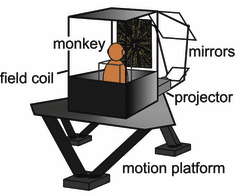
\includegraphics[scale=.4]{apparatus}
  \end{center}
\end{frame}

\begin{frame}
  \frametitle{Mixing weight depends on cue reliability \cite{morgan_multisensory_2008}}
  \begin{center}
    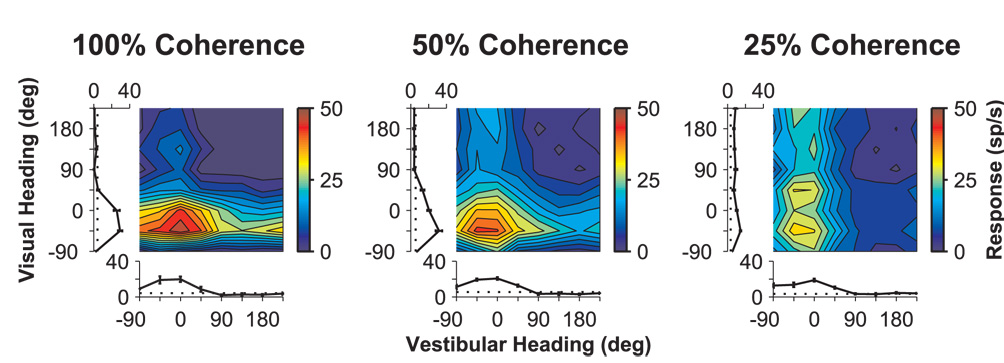
\includegraphics[width=\textwidth]{coherence}

    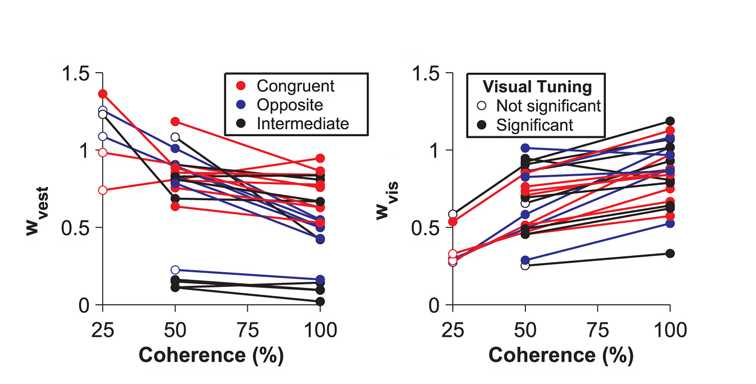
\includegraphics[width=.7\textwidth]{weight}
  \end{center}
\end{frame}

\section{Neural Network Models}

\begin{frame}
  \frametitle{Neural network models}
  \begin{itemize}
    \item Three seemingly isolated studies:
    \begin{itemize}
      \item The psychophysical study of optimal cue integration;
      \item The classical empirical principles of multisensory integration in SC;
      \item The recent neurophysiological findings in MSTd area.
    \end{itemize}

    ~
    \item Two neural network model bridge the gaps:
    \begin{itemize}
      \item The probabilistic population codes for Bayesian inference;
      \item The normalization model.
    \end{itemize}
  \end{itemize}
\end{frame}

\begin{frame}
  \frametitle{Probabilistic population codes (PPCs) \cite{ma_bayesian_2006}}
  \begin{itemize}
    \item A population response activity encodes a Gaussian distribution.
  \end{itemize}
  \begin{center}
    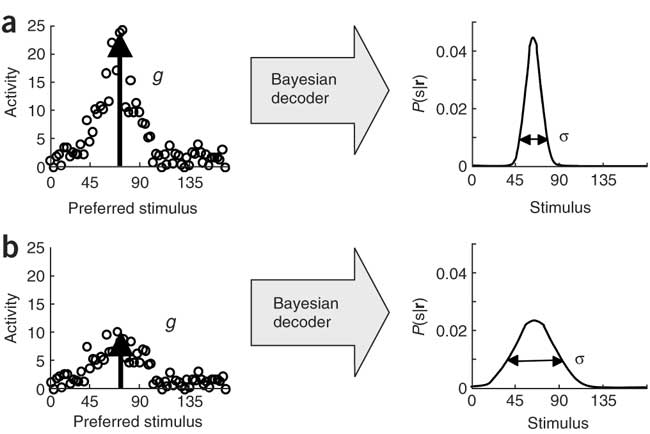
\includegraphics[width=.8\textwidth]{decoder}
  \end{center}
\end{frame}

\begin{frame}
  \frametitle{Probabilistic population codes (PPCs) \cite{ma_bayesian_2006}}
  \begin{itemize}
    \item Poisson variability of neuronal response:
\begin{equation}
  p(\mathbf{r}|s) = \prod_{i} p(r_i|s) = \prod_{i} \frac{e^{-f_i(s)} f_i(s)^{r_i}}{r_i!}
  \label{eq:popvar}
\end{equation}
    \item Consider a multisensory integration task:
    \begin{itemize}
      \item $\mathbf{r}_1$ and $\mathbf{r}_2$ encode the input sensory cues;
      \item Each neuron are aligned with same tuning curve profile.
    \end{itemize}
    \item Bayesian inference can be calculated via sum of the two populations.
    \begin{equation} \mathbf{r}_3 = \mathbf{r}_1 + \mathbf{r}_2 \end{equation}
    \item We can show that
    \begin{equation} p(s|\mathbf{r}_3) = p(s|\mathbf{r}_1,\mathbf{r}_2) \end{equation}
  \end{itemize}
\end{frame}

\begin{frame}
  \frametitle{Probabilistic population codes (PPCs) \cite{ma_bayesian_2006}}
  \begin{itemize}
    \item Bayesian inference using probabilistic population codes.
  \end{itemize}
  \begin{center}
    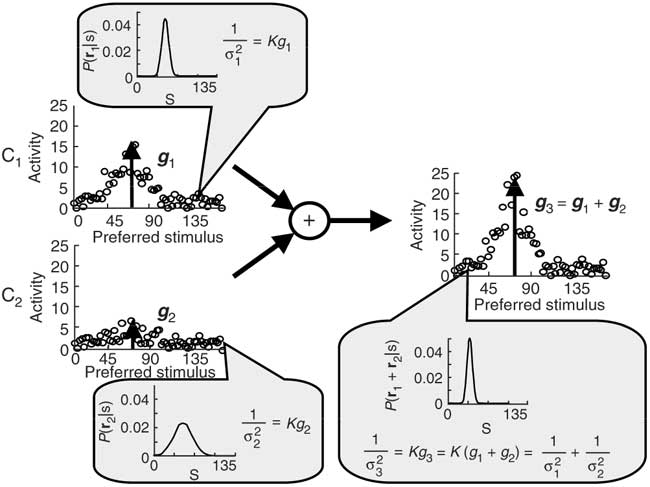
\includegraphics[width=.8\textwidth]{infer}
  \end{center}
\end{frame}

\begin{frame}
  \frametitle{Probabilistic population codes (PPCs) \cite{ma_bayesian_2006}}
  \begin{itemize}
    \item PPCs also works with general assumptions
    \begin{itemize}
      \item Poisson-like variability;
      \item Non-flat prior;
      \item Different tune curves.
    \end{itemize}

    ~
    \item PPCs links neuronal responses to behavior.
    \item It shows a possible case how brain can perform Bayesian computation.
  \end{itemize}
\end{frame}

\begin{frame}
  \frametitle{The normalization model \cite{ohshiro_normalization_2011}}
  \begin{itemize}
    \item A computational model at a network level.
    \item Accounts for both empirical principles and reliability-dependent combination rule.
  \end{itemize}
  \begin{center}
    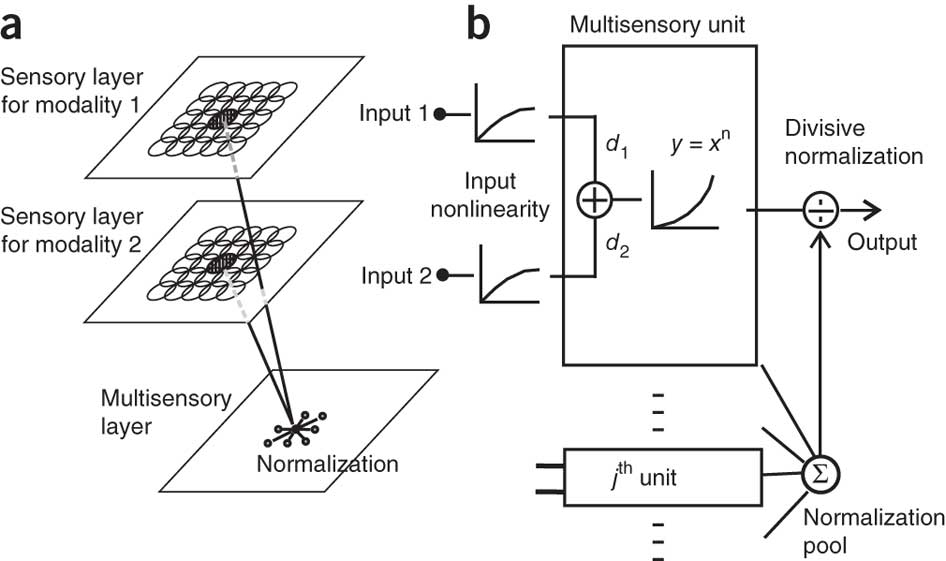
\includegraphics[width=.8\textwidth]{normalize}
  \end{center}
\end{frame}

\begin{frame}
  \frametitle{The normalization model \cite{ohshiro_normalization_2011}}
  \begin{itemize}
    \item Weighted sum of unisensory inputs
\begin{equation}
  E = d_1 I_1(s) + d_1 I_2(s)
  \label{eq:step1}
\end{equation}
    where each multisensory neuron has different dominance weights ($d_1$ and $d_2$).
    \item Normalizing over the whole population activity.
\begin{equation}
  R = \frac{E^n}{\alpha^n+\frac{1}{N}\sum_{j=1}^N E_j^n}
  \label{eq:step2}
\end{equation}
    \item Normalization commonly exists in many brain areas.
  \end{itemize}
\end{frame}


\begin{frame}
  \frametitle{The normalization model accounts for the principle of the ``inverse effectiveness'' \cite{ohshiro_normalization_2011}}
  \begin{center}
    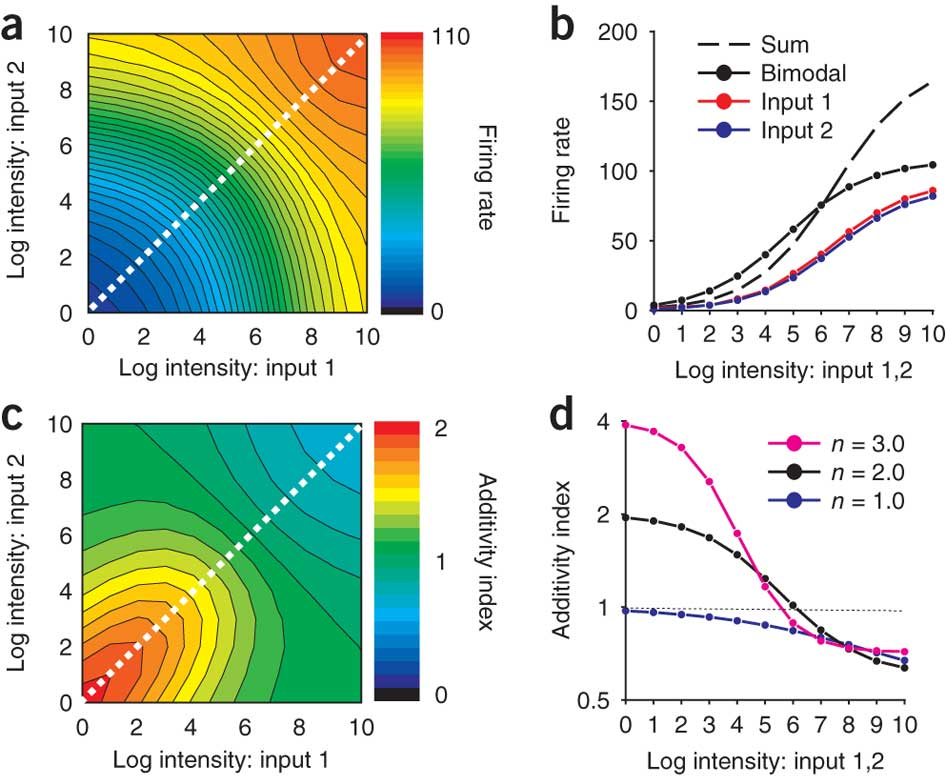
\includegraphics[width=.6\textwidth]{inverse2}
  \end{center}
  \[ Additivity Index = \frac{R_{comb}}{R_1 + R_2} \]
\end{frame}

\begin{frame}
  \frametitle{The normalization model accounts for the ``spatial principle'' \cite{ohshiro_normalization_2011}}
  \begin{center}
    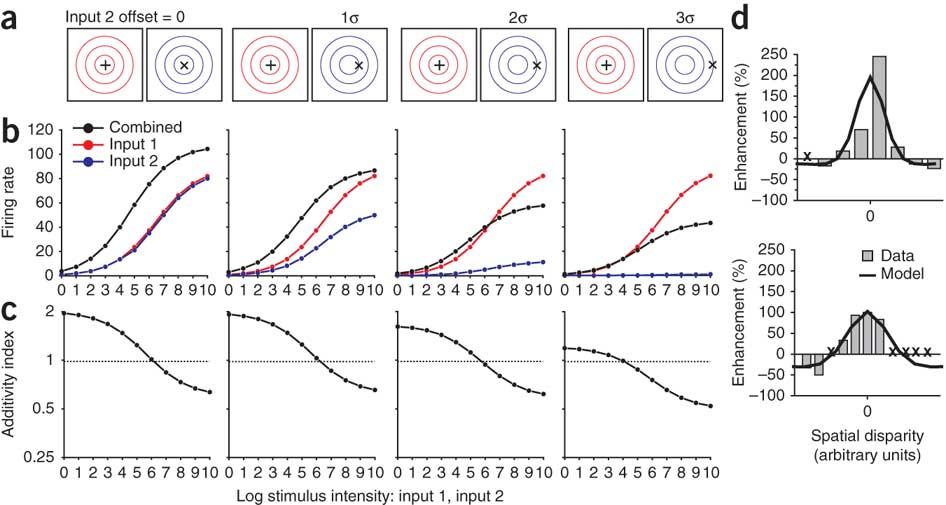
\includegraphics[width=\textwidth]{spatial}
  \end{center}
\end{frame}

\begin{frame}
  \frametitle{The normalization model accounts for reliability-dependent combination rule \cite{ohshiro_normalization_2011}}
  \begin{center}
    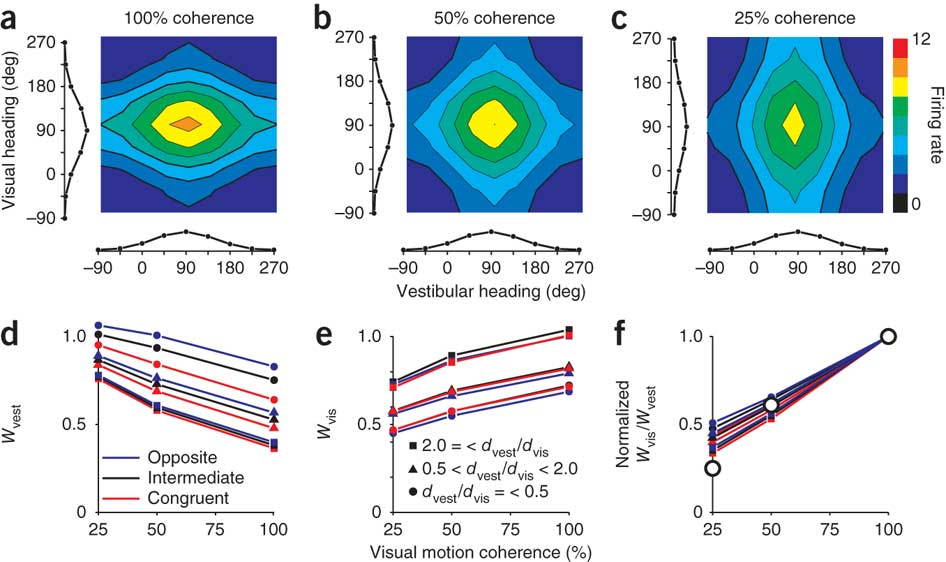
\includegraphics[width=.9\textwidth]{normweight}
  \end{center}
\end{frame}

\section{Discussion}
\begin{frame}
  \frametitle{Discussion}
  \begin{itemize}
    \item Psychophysical study
    \begin{itemize}
      \item Behavioral observation matches normative prediction.
    \end{itemize}
    \item Neurophysiological study
    \begin{itemize}
      \item Empirical principles describe the properties of multisensory neuron.
      \item Reliability-dependent linear combination rule describes the underlying computational mechanism.
    \end{itemize}
    \item Two neural network models:
    \begin{itemize}
      \item PPCs links neuronal response to behavior.
      \item The normalization model is at network level and unifies neurophysiological findings.
    \end{itemize}

    ~
    \item A potential combination of these models will be interesting.
  \end{itemize}
\end{frame}

\begin{frame}
  \frametitle{The end}
  \begin{center}
    \Huge{Thank you!}

    ~

    \Huge{Questions?}
  \end{center}
\end{frame}

\begin{frame}[allowframebreaks]
  \frametitle{References}
  {\footnotesize
  \bibliography{bib}
  \bibliographystyle{apacite}  
  }
\end{frame}


\end{document}
